\documentclass{scrreprt}
\usepackage[utf8]{inputenc}
\usepackage{xcolor}
\usepackage{amsmath,amsthm,amssymb,amsfonts, fancyhdr, color, comment, graphicx, environ}
\usepackage[explicit]{titlesec}
\usepackage{soul}
\usepackage[top=1.8cm, bottom=1.5cm, left=1.5cm, right=1.5cm]{geometry}
\usepackage{karnaugh-map}
\usepackage{booktabs}
\usepackage{mdframed}
\usepackage{fix-cm}
\usepackage{tabularx}
\usepackage{tikz, fouriernc}
\usetikzlibrary{calc}
\usepackage[hidelinks]{hyperref}

\definecolor{lime}{RGB}{0,0,128}
\definecolor{titleblue}{HTML}{4a7aa4}
\setlength{\parindent}{0pt}

\newbox\TitleUnderlineTestBox
\newcommand*\TitleUnderline[1]
  {%
    \bgroup
    \setbox\TitleUnderlineTestBox\hbox{\colorbox{titleblue}\strut}%
    \setul{\dimexpr\dp\TitleUnderlineTestBox-.3ex\relax}{.3ex}%
    \ul{#1}%
    \egroup
  }
\newcommand*\SectionNumberBox[1]
  {%
    \colorbox{titleblue}
      {%
        \makebox[2.5em][c]
          {%
            \color{white}%
            \strut
            \csname the#1\endcsname
          }%
      }%
    \TitleUnderline{\ \ \ }%
  }
\titleformat{\section}
  {\Large\bfseries\sffamily\color{titleblue}}
  {\SectionNumberBox{section}}
  {0pt}
  {\TitleUnderline{#1}}
\titleformat{\subsection}
  {\large\bfseries\sffamily\color{titleblue}}
  {\SectionNumberBox{subsection}}
  {0pt}
  {\TitleUnderline{#1}}
\titleformat{\subsubsection}
  {\normalsize\bfseries\sffamily\color{titleblue}}
  {\SectionNumberBox{subsubsection}}
  {0pt}
  {\TitleUnderline{#1}}

  \definecolor{numbercolor}{gray}{0.7}

  \makeatletter
  \renewcommand\chapterheadstartvskip{\vskip50pt}
  
  \newcommand\chaptitlefont{%
    \fontfamily{pbk}\fontseries{db}%
    \fontshape{n}\fontsize{25}{35}\selectfont\raggedleft}
  
  \newcommand\chapnumfont{%
    \fontfamily{pbk}\fontseries{m}\fontshape{n}%
    \fontsize{1in}{0in}\selectfont\color{titleblue}}
  
  \renewcommand\chapterheadendvskip{\par\vskip2mm\hrule\vskip40pt}
  
  \renewcommand*{\@@makechapterhead}[1]{\chapterheadstartvskip
    {%
      \setlength{\parindent}{\z@}\setlength{\parfillskip}{\fill}%
      \normalfont\sectfont\nobreak\size@chapter{}%
      \if@chapterprefix
        \let\@tempa\raggedsection
      \else
        \let\@tempa\@hangfrom
      \fi
      \@tempa{\ifnum \c@secnumdepth >\m@ne%
            \if@chapterprefix
              \expandafter\size@chapterprefix
            \else
              \expandafter\size@chapter
            \fi
            \if@chapterprefix
              \size@chapterprefix{}\endgraf\nobreak\vskip.5\baselineskip
            \fi
        \fi
      }%
  \begin{tabularx}{\textwidth}{Xl}
  {\parbox[b]{\linewidth}{\chaptitlefont #1}}
  & \raisebox{-15pt}{\chapnumfont\thechapter}%
  \end{tabularx}%
   \nobreak\chapterheadendvskip
  }%
  }
  \renewcommand*{\@@makeschapterhead}[1]{%
    \chapterheadstartvskip%
    {\normalfont\sectfont\nobreak\size@chapter{}%
      \setlength{\parindent}{\z@}\setlength{\parfillskip}{\fill}%
      \raggedsection \interlinepenalty \@M 
  \begin{tabularx}{\textwidth}{X}%
  {\parbox[b]{\linewidth}{\chaptitlefont #1}%
  \vphantom{\raisebox{-15pt}{\chapnumfont 1}}}
  \end{tabularx}%
  \par}%
    \nobreak\chapterheadendvskip%
  }
  \makeatother

\pagestyle{fancy}
\fancyhf{}
\renewcommand{\headrulewidth}{0.4pt}
\renewcommand{\footrulewidth}{0pt}
\fancyhead[L]{\textbf{Villar Pedro}}
\fancyhead[R]{\textbf{FaMAF, Org. del Computador}}
\fancyhead[C]{\thepage}

%% Cambiar nombre de la tabla de contenidos

\begin{document}

%-------------------------------------------%
% Portada del documento
\begin{titlepage}
  \begin{tikzpicture}[overlay,remember picture]
      \fill[lime!10] (current page.south east) rectangle (current page.north west);
      \fill[lime,even odd rule] (current page.south west) rectangle ([xshift=1.5cm]current page.north west) ($(current page.north west)!.5!(current page.south west)$) arc(180:270:3) ($(current page.north west)!.5!(current page.south west)$) arc(270:450:3.5) ([yshift=7cm]$(current page.north west)!.5!(current page.south west)$)  arc(180:90:3);
%           \draw[lime!10,double=lime!10,double distance=2mm] (current page.south west) --+ (2,2) --+ (-2,6) --+ (2,8) --+ (-2,9) --+ (2,13) --+ (-2,18) --+ (2,30);
          \draw[lime,thin] (13,-1) node[lime,above left] {\Huge Org. del Computador} --+ (0,3) node[lime,below right] {\Huge 1C-2024};
      \node[yshift=-5cm,xslant=1,yscale=1.6,lime!40,opacity=.2] at (9.5,-6.5) {\scalebox{6}{Apunte}};
      \node[yshift=-5cm,lime] at (8,-7) {\scalebox{6}{Apunte}};
          \draw[lime,fill=titleblue!20] ([xshift=-1cm]current page.north east) -- ([yshift=-1cm]current page.north east) -- ([yshift=-2cm]current page.north east) -- ([xshift=-2cm]current page.north east);
      \path ([xshift=-1cm]current page.north east) -- ([yshift=-1cm]current page.north east) node[midway,sloped,below=.1cm,lime] {Villar Pedro};
  \end{tikzpicture}
\end{titlepage}
%-------------------------------------------%

\tableofcontents
\newpage

\listoffigures
\newpage
%-------------------------------------------%
\chapter{Primer Parcial}

\textbf{Fecha:} 24/04/2024
\vspace{1cm}

\textbf{Prácticos:} 1, 2, 3, 4 y 5.
\vspace{1cm}

\textbf{Temas:}
\begin{itemize}
    \item \hyperref[sec:num]{Sistemas de Numeración.}
    \item \hyperref[sec:bool]{Álgebra de Boole.}
    \item \hyperref[sec:logica]{Lógica Combinacional.}
    \item \hyperref[sec:mem]{Direccionamiento y Lógica de Decodificación de Memorias.}
    \item \hyperref[sec:sec]{Circuitos secuenciales.}
\end{itemize}

\newpage  
%-------------- Sistemas de Numeración --------------%
\section{Sistemas de Numeración}\label{sec:num}
\documentclass[20pt,margin=1in,innermargin=-4.5in,blockverticalspace=-0.25in]{tikzposter}
\geometry{paperwidth=42in,paperheight=30in}
\usepackage[utf8]{inputenc}
\usepackage{amsmath}
\usepackage{amsfonts}
\usepackage{amsthm}
\usepackage{amssymb}
\usepackage{mathrsfs}
\usepackage{graphicx}
\usepackage{adjustbox}
\usepackage{enumitem}
\usepackage[backend=biber,style=numeric]{biblatex}
\usepackage{emory-theme}
\usepackage{emory-theme}
\usepackage{mwe} % for placeholder images
\usepackage{booktabs}
% set theme parameters
\tikzposterlatexaffectionproofoff
\usetheme{EmoryTheme}
\usecolorstyle{EmoryStyle}

\title{Sistema IEEE 754 - Precisión Simple}
\author{Pedro Villar}
\institute{Organización del Computador - Primer Cuatrimestre 2024}	
\titlegraphic{\adjustbox{left=0.35\textwidth}{
\includegraphics[width=0.3\textwidth]{famaf-logo.jpg}}}

% begin document
\begin{document}
\maketitle
\centering
\block{¿Qué es el sistema IEEE 754?}{
        El sistema IEEE 754 es un estándar para la representación de números en punto flotante. Este sistema establece las caracteristicas de las tres partes de un número en punto flotante: el \textbf{signo}, \textbf{exponente} y \textbf{fracción (mantisa)}. Se enfoca en el método de precisión simple que utiliza 32 bits.
    }
\begin{columns}
    \column{0.5}
    \block{Características}{
        \begin{center} \textbf{Bit de signo:} \end{center}
        El bit de signo es el primer bit del número en punto flotante. \textbf{Si el bit de signo es 0}, el número es \textbf{positivo}, \textbf{si es 1}, el número es \textbf{negativo}.    
        \begin{center} \textbf{Exponente:} \end{center}
        Indica cuántos “lugares” se debe desplazar hacia la derecha o hacia la izquierda la coma binaria de la parte significativa. El exponente de un número puede ser tanto positivo como negativo. En el caso de la precisión simple, el exponente se representa con 8 bits y se suma 127 al valor del exponente para obtener el valor.
        \begin{center} \textbf{Mantisa o parte fraccionaria:} \end{center}
        La mantisa es la parte fraccionaria del número en punto flotante. En el caso de la precisión simple, la mantisa se representa con 23 bits. Debe ser normalizada, eso se logra moviendo la coma binaria a la izquierda hasta que el primer bit sea 1.
        \begin{equation*}
            1,xxxxx \times 2^{yyyy}
        \end{equation*}
        Al hacer esto, se debe adaptar el exponente para que el valor no se modifique, es decir, el exponente será ahora \textbf{la cantidad de veces que se movió la coma binaria a la izquierda}.
    }

    \block{Convertir de decimal a IEEE 754}{
        \begin{enumerate}
            \item Determinar el bit de signo.
            \item Convertir la parte entera y la parte fraccionaria a binario.
            \item Normalizar.
            \item Encontrar el exponente moviendo la coma y sumando 127, expresado en binario.
            \item Encontrar la parte fraccionaria.
            \item Conformar el número en punto flotante.
        \end{enumerate}
    }
    \block{Convertir de IEEE 754 a decimal}{
        \begin{enumerate}
            \item Dividir el número en punto flotante en sus tres partes.
            \item Encontrar el bit de signo.
            \item Encontrar el exponente y restarle 127.
            \item Desnormalizar el número y pasarlo a decimal.
        \end{enumerate}
    }
    
    \column{0.5}
    \block{Ejemplo de conversión de decimal a IEEE 754}{
        Se busca convertir el número $723.125_{10}$ a IEEE 754.
        \begin{enumerate}
            \item El bit de signo es 0, ya que el número es positivo.
            \item Se convierte la parte entera y la parte fraccionaria a binario.
            \begin{itemize}
                \item Parte entera:
                \begin{align*}
                    723 \div 2 &= 361 \text{ residuo } 1 \\
                    361 \div 2 &= 180 \text{ residuo } 1 \\
                    180 \div 2 &= 90 \text{ residuo } 0 \\
                    90 \div 2 &= 45 \text{ residuo } 0 \\
                    45 \div 2 &= 22 \text{ residuo } 1 \\
                    22 \div 2 &= 11 \text{ residuo } 0 \\
                    11 \div 2 &= 5 \text{ residuo } 1 \\
                    5 \div 2 &= 2 \text{ residuo } 1 \\
                    2 \div 2 &= 1 \text{ residuo } 0 \\
                    1 \div 2 &= 0 \text{ residuo } 1 \\
                \end{align*}
                Por lo que la parte entera en binario es $1011010011$.
                \item Parte fraccionaria:
                \begin{align*}
                    0.125 \times 2 &= 0.25 \\
                    0.25 \times 2 &= 0.5 \\
                    0.5 \times 2 &= 1
                \end{align*}
                Por lo que la parte fraccionaria en binario es $001$.
            \end{itemize}
            El número en binario es $1011010011.001$.
            \item Para normalizar movemos la coma tantos lugares como sea necesario para que quede un uno seguido por una parte fraccionaria.
            \begin{itemize}
                \item \textbf{Sin normalizar:} $1011010011.001 \times 2^0$
                \item \textbf{Normalizado:} $1.011010011001 \times 2^{10}$
            \end{itemize}
            \item El exponente es la cantidad de veces que se movió la coma binaria a la izquierda, en este caso, 10 veces. Por lo que el exponente es $127 + 10 = 137_{10} = 10001001_2$.
            \item La parte fraccionaria se compone por los 23 bits que siguen a la coma decimal del número normalizado.
            \begin{equation*}
                01101001100100000000000
            \end{equation*}
            \item Para conformar el número en punto flotante, se coloca el bit de signo, el exponente y la parte fraccionaria.
            \begin{equation*}
                0 \ 10001001 \ 01101001100100000000000
            \end{equation*}
        \end{enumerate}   
    }
\end{columns}

\end{document}
%-------------------------------------------------%

\newpage
%-------------- Álgebra de Boole --------------%
\section{Álgebra de Boole}\label{sec:bool}
\documentclass[20pt,margin=1in,innermargin=-4.5in,blockverticalspace=-0.25in]{tikzposter}
\geometry{paperwidth=42in,paperheight=30in}
\usepackage[utf8]{inputenc}
\usepackage{amsmath}
\usepackage{amsfonts}
\usepackage{amsthm}
\usepackage{amssymb}
\usepackage{mathrsfs}
\usepackage{graphicx}
\usepackage{adjustbox}
\usepackage{enumitem}
\usepackage[backend=biber,style=numeric]{biblatex}
\usepackage{emory-theme}
\usepackage{emory-theme}
\usepackage{mwe} % for placeholder images
\usepackage{booktabs}
% set theme parameters
\tikzposterlatexaffectionproofoff
\usetheme{EmoryTheme}
\usecolorstyle{EmoryStyle}

\title{Sistema IEEE 754 - Precisión Simple}
\author{Pedro Villar}
\institute{Organización del Computador - Primer Cuatrimestre 2024}	
\titlegraphic{\adjustbox{left=0.35\textwidth}{
\includegraphics[width=0.3\textwidth]{famaf-logo.jpg}}}

% begin document
\begin{document}
\maketitle
\centering
\block{¿Qué es el sistema IEEE 754?}{
        El sistema IEEE 754 es un estándar para la representación de números en punto flotante. Este sistema establece las caracteristicas de las tres partes de un número en punto flotante: el \textbf{signo}, \textbf{exponente} y \textbf{fracción (mantisa)}. Se enfoca en el método de precisión simple que utiliza 32 bits.
    }
\begin{columns}
    \column{0.5}
    \block{Características}{
        \begin{center} \textbf{Bit de signo:} \end{center}
        El bit de signo es el primer bit del número en punto flotante. \textbf{Si el bit de signo es 0}, el número es \textbf{positivo}, \textbf{si es 1}, el número es \textbf{negativo}.    
        \begin{center} \textbf{Exponente:} \end{center}
        Indica cuántos “lugares” se debe desplazar hacia la derecha o hacia la izquierda la coma binaria de la parte significativa. El exponente de un número puede ser tanto positivo como negativo. En el caso de la precisión simple, el exponente se representa con 8 bits y se suma 127 al valor del exponente para obtener el valor.
        \begin{center} \textbf{Mantisa o parte fraccionaria:} \end{center}
        La mantisa es la parte fraccionaria del número en punto flotante. En el caso de la precisión simple, la mantisa se representa con 23 bits. Debe ser normalizada, eso se logra moviendo la coma binaria a la izquierda hasta que el primer bit sea 1.
        \begin{equation*}
            1,xxxxx \times 2^{yyyy}
        \end{equation*}
        Al hacer esto, se debe adaptar el exponente para que el valor no se modifique, es decir, el exponente será ahora \textbf{la cantidad de veces que se movió la coma binaria a la izquierda}.
    }

    \block{Convertir de decimal a IEEE 754}{
        \begin{enumerate}
            \item Determinar el bit de signo.
            \item Convertir la parte entera y la parte fraccionaria a binario.
            \item Normalizar.
            \item Encontrar el exponente moviendo la coma y sumando 127, expresado en binario.
            \item Encontrar la parte fraccionaria.
            \item Conformar el número en punto flotante.
        \end{enumerate}
    }
    \block{Convertir de IEEE 754 a decimal}{
        \begin{enumerate}
            \item Dividir el número en punto flotante en sus tres partes.
            \item Encontrar el bit de signo.
            \item Encontrar el exponente y restarle 127.
            \item Desnormalizar el número y pasarlo a decimal.
        \end{enumerate}
    }
    
    \column{0.5}
    \block{Ejemplo de conversión de decimal a IEEE 754}{
        Se busca convertir el número $723.125_{10}$ a IEEE 754.
        \begin{enumerate}
            \item El bit de signo es 0, ya que el número es positivo.
            \item Se convierte la parte entera y la parte fraccionaria a binario.
            \begin{itemize}
                \item Parte entera:
                \begin{align*}
                    723 \div 2 &= 361 \text{ residuo } 1 \\
                    361 \div 2 &= 180 \text{ residuo } 1 \\
                    180 \div 2 &= 90 \text{ residuo } 0 \\
                    90 \div 2 &= 45 \text{ residuo } 0 \\
                    45 \div 2 &= 22 \text{ residuo } 1 \\
                    22 \div 2 &= 11 \text{ residuo } 0 \\
                    11 \div 2 &= 5 \text{ residuo } 1 \\
                    5 \div 2 &= 2 \text{ residuo } 1 \\
                    2 \div 2 &= 1 \text{ residuo } 0 \\
                    1 \div 2 &= 0 \text{ residuo } 1 \\
                \end{align*}
                Por lo que la parte entera en binario es $1011010011$.
                \item Parte fraccionaria:
                \begin{align*}
                    0.125 \times 2 &= 0.25 \\
                    0.25 \times 2 &= 0.5 \\
                    0.5 \times 2 &= 1
                \end{align*}
                Por lo que la parte fraccionaria en binario es $001$.
            \end{itemize}
            El número en binario es $1011010011.001$.
            \item Para normalizar movemos la coma tantos lugares como sea necesario para que quede un uno seguido por una parte fraccionaria.
            \begin{itemize}
                \item \textbf{Sin normalizar:} $1011010011.001 \times 2^0$
                \item \textbf{Normalizado:} $1.011010011001 \times 2^{10}$
            \end{itemize}
            \item El exponente es la cantidad de veces que se movió la coma binaria a la izquierda, en este caso, 10 veces. Por lo que el exponente es $127 + 10 = 137_{10} = 10001001_2$.
            \item La parte fraccionaria se compone por los 23 bits que siguen a la coma decimal del número normalizado.
            \begin{equation*}
                01101001100100000000000
            \end{equation*}
            \item Para conformar el número en punto flotante, se coloca el bit de signo, el exponente y la parte fraccionaria.
            \begin{equation*}
                0 \ 10001001 \ 01101001100100000000000
            \end{equation*}
        \end{enumerate}   
    }
\end{columns}

\end{document}
%-------------------------------------------------%

\newpage
%-------------- Lógica Combinacional --------------%
\section{Lógica Combinacional}\label{sec:logica}
Una unidad de memoria es un conjunto de celdas de almacenamiento junto con los circuitos asociados que se requieren para transferir información al y del dispositivo. El tiempo que toma transferir información a o de cualquier posición al azar deseada siempre es el mismo, de ahí el nombre memoria de acceso aleatorio o RAM

Una unidad de memoria almacena información binaria en grupos de bits llamados \textbf{palabras}. Una palabra de memoria es una \textit{entidad de bits que siempre se guardan o sacan juntos}, como una unidad. Una palabra de memoria es un \textit{grupo de unos y ceros y podría representar un número, una instrucción, uno o más caracteres alfanuméricos o cualquier otra información codificada en binario}. Un grupo de ocho bits es un byte. Casi todas las memorias de computadora manejan palabras \textbf{cuya longitud es un múltiplo de ocho bits}. Así, una palabra de 16 bits contiene dos bytes, y una de 32 bits consta de cuatro bytes. La capacidad de una unidad de memoria por lo regular se da como el número total de bytes que es capaz de guardar.

\subsection{Comunicación con la Memoria}
La comunicación entre la memoria y su entorno se efectúa a través de líneas de entrada y salida de datos, líneas de selección de direcciones y líneas de control que especifican la dirección de la transferencia.

Las $n$ líneas de entrada de datos alimentan la información que se guardará en la memoria, y las $n$ líneas de salida de datos proporcionan la información que viene de la memoria. Las $k$ líneas de dirección especifican la palabra específica escogida, de entre muchas disponibles. Las dos entradas de control especifican la dirección de la transferencia deseada: la entrada de escritura hace que se transfieran datos binarios a la memoria; la de lectura hace que se saquen datos binarios de la memoria.

\begin{figure}[h]
\centering
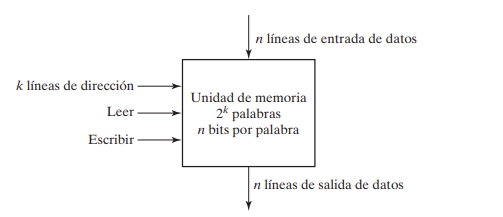
\includegraphics[scale=0.95]{img/mem.png}
\caption{Diagrama de bloques - Unidad de Memoria}
\end{figure}

La unidad de memoria se especifica con el número de palabras que contiene y el número de bits que hay en cada palabra. Las líneas de dirección seleccionan una palabra específica. A cada palabra de la memoria se asigna un número de identificación, llamado dirección, entre $0$ y $2^k -1$, donde $k$ es el número de líneas de dirección. La selección de una palabra específica de la memoria se efectúa aplicando los $k$ bits de dirección a las líneas de dirección. Un decodificador acepta esta dirección y abre las trayectorias necesarias para seleccionar la palabra especificada.

Para nombrar a las memorias, se suele decir que es de una capacidad y de tantos bits. La capacidad de palabras (o bytes) de la memoria se da con letras tales como: $K$ (kilo), $M$ (mega), $G$ (giga), $T$ (tera). $K$ es igual a $2^{10}$, $M$ es igual a $2^{20}$, $G$ es igual a $2^{30}$ y $T$ es igual a $2^{40}$.

\begin{mdframed}[backgroundcolor=gray!10,linewidth=0]
    Por ejemplo, la unidad de memoria con capacidad de 1K palabras de 16 bits cada una. Puesto que 1K=1024=210 y 16 bits constituyen dos bytes, se afirma que la memoria puede dar cabida a 2048=2K bytes.
\end{mdframed}

\newpage
El diagrama correspondiente a una memoria de $1K$ palabras de $16$ bits cada una se muestra en la figura \ref{fig:memfoto}.
\begin{figure}[h]
\centering
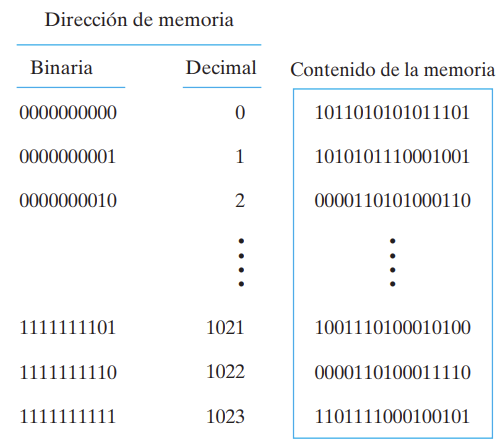
\includegraphics[scale=0.7]{img/ejem.png}
\caption{Contenido de una memoria de 1024 x 16}
\label{fig:memfoto}
\end{figure}

Cada palabra contiene 16 bits que se
dividen en dos bytes. Las palabras se reconocen por su dirección decimal, de 0 a 1023. La dirección binaria equivalente consta de 10 bits. La primera dirección se especifica con 10 ceros, y la última, con 10 unos. Ello se debe a que 1023 en binario es 1111111111. Seleccionamos una palabra de memoria por su dirección binaria. Cuando se lee o escribe una palabra, la memoria opera sobre los 16 bits como una sola unidad.

\begin{mdframed}[backgroundcolor=gray!10,linewidth=0]
    La memoria de $1K \times 16$ de la figura \ref{fig:memfoto} tiene $10$ bits en la dirección y $16$ bits en cada palabra.
\end{mdframed}

\subsection{Mapas de Karnaugh}
\begin{mdframed}[backgroundcolor=gray!10,linewidth=0]
    Los mapas de Karnaugh son una herramienta útil que nos permite aplicar un método de simplificación de funciones lógicas.
\end{mdframed}

El Mapa de Karnaugh tiene la característica de que puede ser visto como una representación bidimensional de una tabla de verdad. En la tabla de verdad, se colocan las variables por columnas y las combinaciones de tales variables determinan un valor de salida, 0 o 1, sin embargo, en el mapa las variables se colocan como si de un plano cartesiano se tratara, respetando cada una de las combinaciones que de ellas se generan, y colocando en la intersección de las combinaciones de las variables, el valor de salida.


\newpage
\begin{figure}[h]
    \centering
    \begin{karnaugh-map}[4][4][1][$w$][$z$][$y$][$x$]
        \minterms{0,1,2,3,4,8,9,11,12}
        \autoterms[0]
        \implicant{0}{8}{red}
        \implicant{0}{2}{blue}
        \implicant{0}{1}{green}
    \end{karnaugh-map}
    \caption{Ejemplo de un mapa de Karnaugh}
\end{figure}

Los mapas muestran la relación que existe entre  las entradas y las salidas de un circuito lógico, si se aplica adecuadamente el resultado será el más simplificado posible. Pueden ser utilizados para cualquier número de variables de entrada sin embargo se recomienda un máximo de seis variables.

\subsubsection{Representación de tabla de verdad en un mapa de Karnaugh}

Las tablas de la verdad se pueden representar en un mapa de Karnaugh, para ello se deben seguir los siguientes pasos:
\begin{enumerate}
    \item Se deben identificar los términos de la tabla de verdad que son 1.
    \item Se deben identificar los términos de la tabla de verdad que son 0.
    \item Se deben identificar los términos de la tabla de verdad que son 1 y que se pueden agrupar.
    \item Se deben identificar los términos de la tabla de verdad que son 0 y que se pueden agrupar.
\end{enumerate}

\begin{mdframed}[backgroundcolor=gray!10,linewidth=0]
    Observaciones:
    \begin{itemize}
        \item Los términos de la tabla de verdad que son 1 se representan en el mapa de Karnaugh con un $1$, y sirven para expresar a la función como una suma de productos.
        \item Los términos de la tabla de verdad que son 0 se representan en el mapa de Karnaugh con un $0$ y sirven para expresar a la función como un producto de sumas.
    \end{itemize}
\end{mdframed}

\newpage
\subsubsection{Ejemplo de representación de tabla de verdad en un mapa de Karnaugh}

Supongamos que se tiene la siguiente tabla de la verdad:

\begin{table}[h]
    \centering
    \begin{tabular}{ccccc}
        \toprule
        \textbf{x} & \textbf{y} & \textbf{z} & \textbf{w} & \textbf{S}\\
        \midrule
        0 & 0 & 0 & 0 & 0\\
        0 & 0 & 0 & 1 & 1\\
        0 & 0 & 1 & 0 & 1\\
        0 & 0 & 1 & 1 & 0\\
        0 & 1 & 0 & 0 & 1\\
        0 & 1 & 0 & 1 & 0\\
        0 & 1 & 1 & 0 & 0\\
        0 & 1 & 1 & 1 & 1\\
        1 & 0 & 0 & 0 & 1\\
        1 & 0 & 0 & 1 & 0\\
        1 & 0 & 1 & 0 & 0\\
        1 & 0 & 1 & 1 & 1\\
        1 & 1 & 0 & 0 & 0\\
        1 & 1 & 0 & 1 & 1\\
        1 & 1 & 1 & 0 & 1\\
        1 & 1 & 1 & 1 & 0\\
        \bottomrule
    \end{tabular}
\end{table}
Para hacer un mapa de Karnaugh, primero se separan las variabes $xy$ y $zw$ y se colocan en el mapa de la siguiente forma:

\begin{figure}[h]
    \centering
    \begin{karnaugh-map}[4][4][1][$w$][$z$][$y$][$x$]
        %\minterms{3,4,5,6,7,9,12,13,14}
        \autoterms[-]
    \end{karnaugh-map}
    \caption{Mapa de Karnaugh para las variables $xy$}
\end{figure}

\newpage
Luego identificamos los términos de la tabla de verdad que son 1 y los colocamos en el mapa de Karnaugh.
\newline Por ejemplo esta linea de la tabla
\begin{table}[h]
    \centering
    \begin{tabular}{ccccc}
        \toprule
        \textbf{x} & \textbf{y} & \textbf{z} & \textbf{w} & \textbf{S}\\
        \midrule
        0 & 0 & 0 & 1 & 1\\
        \bottomrule
    \end{tabular}
\end{table}

Se coloca en el mapa de Karnaugh en la posición donde $xy$ toma $00$ y $zw$ toma $01$.

\begin{figure}[h]
    \centering
    \begin{karnaugh-map}[4][4][1][$w$][$z$][$y$][$x$]
        \minterms{1}
        \autoterms[0]
        \implicant{1}{1}{red}
    \end{karnaugh-map}
    \caption{Ejemplo de representación}
\end{figure}

Pasar por cada linea de la tabla de verdad y colocar los términos en el mapa de Karnaugh. Los términos que no son $1$ se colocan como $0$ en el mapa de Karnaugh.

\begin{figure}[h]
    \centering
    \begin{karnaugh-map}[4][4][1][$x$][$y$][$z$][$w$]
        \minterms{1,2,4,7,8,11,13,14}
        \autoterms[0]
    \end{karnaugh-map}
    \caption{Mapa de Karnaugh completo del ejemplo.}
\end{figure}

\subsubsection{Agrupación de términos}

Para simplificar la función lógica, se deben agrupar los términos que son 1 en el mapa de Karnaugh. Los términos se pueden agrupar siguiendo las siguientes reglas:

\begin{enumerate}
    \item Los grupos deben contener una cantidad de elementos igual a potencias de 2. Es decir, los grupos solo podrán realizarse con cantidades de celdas iguales a: 1, 2, 4, 8, 16, 32, etc.
    \item Se deben generar grupos con combinaciones de variables adyacentes, es decir, sólo debe de haber un cambio entre cada una de las combinaciones, por ejemplo la combinación $ABC'$ es adyacente con $AB'C'$ , ya que sólo cambia la variable $B$.
    \item Grupos en las posiciones en los extremos y esquinas del mapa. Las posiciones de los extremos y las esquinas son adyacentes, por lo que se pueden agrupar. Esta adyacencia se debe a que el mapa de Karnaught puede ser visto como un toroide.
    \item Grupos de unos darán lugar a una suma de productos o mini términos.
    \item Grupos de ceros darán lugar a un producto de sumas o maxi términos.
    \item Los grupos deben ser lo más grande posible. Se buscará realizar grupos con la mayor cantidad de elementos posibles, entre más grande el grupo, se obtiene una función más simplificada. 
    \item No se pueden generar grupos en diagonal. Solo se permitirán grupos en vertical y horizontal dentro del mapa.
    \item Puede existir solapamiento de grupos, siempre y cuando exista al menos un elemento que no haya sido agrupado anteriormente.
    \item No deben existir grupos redundantes, es decir, no se puede realizar un grupo dentro de otro grupo, y no se puede realizar un grupo con elementos que ya hayan sido completamente agrupados en otros conjuntos.
\end{enumerate}

Por ejemplo, si se tiene este mapa de Karnaugh:

\begin{figure}[h]
    \centering
    \begin{karnaugh-map}[4][4][1][$x$][$y$][$z$][$w$]
        \minterms{4,12,6,14,0,2}
        \autoterms[0]
    \end{karnaugh-map}
    \caption{Mapa de Karnaugh para agrupar.}
\end{figure}

Se debería agrupar de la siguiente forma:

\begin{figure}[h]
    \centering
    \begin{karnaugh-map}[4][4][1][$w$][$z$][$y$][$x$]
        \minterms{4,12,6,14,0,2}
        \autoterms[0]
        \implicantedge{0}{4}{2}{6}{green}
        \implicantedge{4}{12}{6}{14}{red}
    \end{karnaugh-map}
    \caption{Mapa de Karnaugh agrupado.}
    \label{fig:karnaugh_agrupado}
\end{figure}

\newpage
\subsubsection{Simplificación de la función lógica}
Para la simplificación de la función lógica, se usan los grupos que se han formado en el mapa de Karnaugh. Cada grupo se convierte en un término de la función lógica, y se deben sumar los términos que se obtienen de los grupos, teniendo en cuenta lo siguiente:

\begin{enumerate}
    \item Si un grupo es de una sola celda, se incluye igualmente en la función lógica.
    \item En el grupo, las variables que cambian de valor "se me van" del término, y las que no cambian su valor permanecen.
    \item Si un grupo se solapa con otro, no cambia la forma de trabajarlos, cada grupo es un término distinto.
\end{enumerate}

Por ejemplo, tomando el mapa de Karnaugh anterior, se obtiene la siguiente función lógica:
\begin{equation*}
    F = x'w' + yw'
\end{equation*}


\subsection{PLA (Programmable Logic Array)}
Programmable Logic Array (PLA) es un dispositivo lógico de arquitectura fija con puertas AND programables seguidas de puertas OR programables. PLA es básicamente un tipo de dispositivo lógico programable que se utiliza para construir un circuito digital reconfigurable. La estructura de un PLA es la siguiente:

\begin{figure}[h]
    \centering
    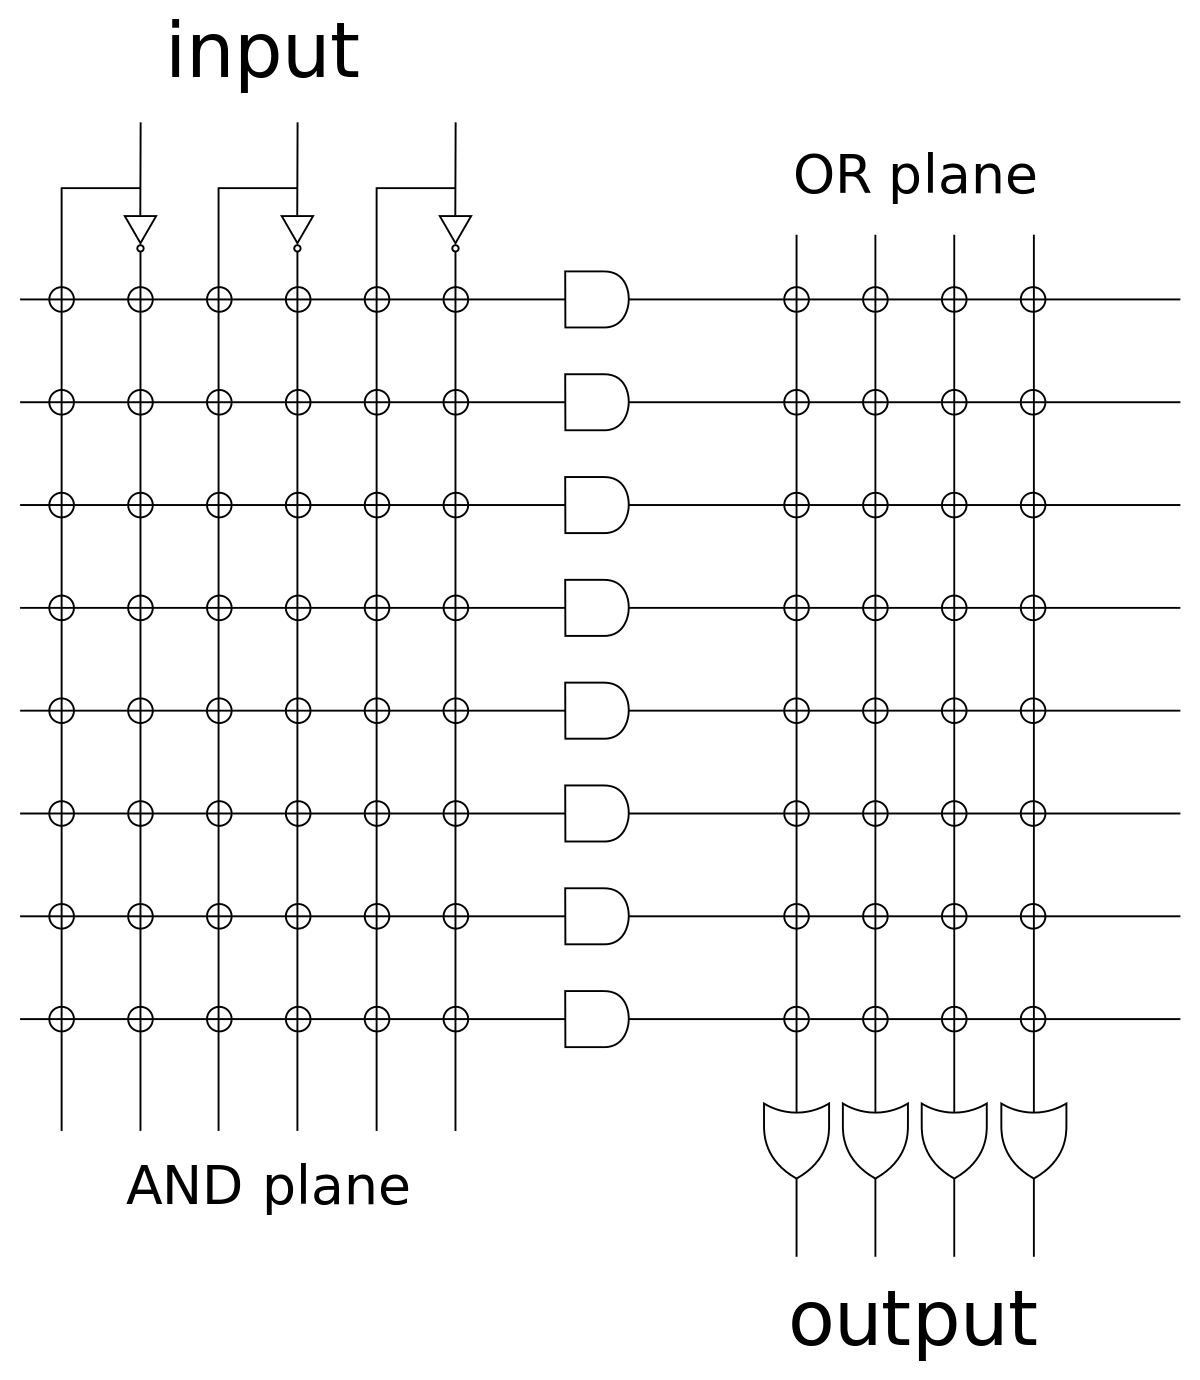
\includegraphics[scale=0.2]{img/pla.png}
    \caption{Estructura de un PLA}
\end{figure}

El funcionamiento se podria resumir en tres pasos:

\begin{enumerate}
    \item \textbf{Programación:} el usuario define la función lógica que se desea implementar.
    \item \textbf{Generación de términos del producto:} las entradas se aplican a la matriz de puertas AND para producir un conjunto de términos de producto.
    \item \textbf{Generación de suma de términos:} los términos de producto se aplican a la matriz de puertas OR para producir la salida.
\end{enumerate}

\newpage
\subsubsection{Método para implementar una función lógica en un PLA}
\begin{mdframed}[backgroundcolor=gray!10,linewidth=0]
    \begin{enumerate}
        \item Una vez se tenga la función lógica simplificada, se deben identificar los términos de la función.
        \item Cada término de la función se convierte en una fila de la matriz de puertas AND.
        \item Luego se suman los términos de la función y se convierten en una fila de la matriz de puertas OR.
        \item La salida de la matriz de puertas OR es la función lógica implementada en el PLA.
    \end{enumerate}
\end{mdframed}


\subsection{Construcción de memorias}
Cuando surge la pregunta: ¿Cuantos chips de memoria se necesitan para almacenar $1K$ palabras de $16$ bits cada una? La respuesta es: $1K \times 16 = 16K$ bits. Si cada chip de memoria tiene $1K$ bits, entonces se necesitan $16$ chips.

\begin{mdframed}[backgroundcolor=gray!10,linewidth=0]
    Para generalizar, si se tienen $m$ palabras de $n$ bits cada una, se necesitan $m \times n$ bits. Si cada chip de memoria tiene $k$ bits, entonces se necesitan $\frac{m \times n}{k}$ chips.
\end{mdframed}

\newpage
\subsubsection{Tamaño de la memoria y dirección}
La cantidad de bits de una memoria se calcula como $2^{\text{dirección}} \times \text{tamaño de palabra}$. Por ejemplo, si se tiene una memoria de $16$ palabras de $8$ bits cada una, la cantidad de bits de la memoria es $2^4 \times 8 = 128$ bits. 

Generalmente el gráfico de una memoria se representa de la siguiente manera:

\begin{figure}[h]
    \centering
    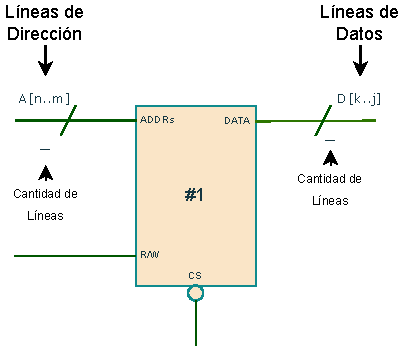
\includegraphics[scale=1]{img/diagramamem.pdf}
    \caption{Diagrama de una memoria}
\end{figure}
Donde de la cantidad de líneas de dirección se obtiene la cantidad de palabras y de la cantidad de líneas de datos se obtiene el tamaño de la palabra.


\subsection{Ampliación de palabra}
Para ampliar la palabra de una memoria, se debe agregar un chip de memoria adicional. Por ejemplo, si se tiene una memoria de $1k$ palabras de $8$ bits cada una y se desea ampliar la palabra a $16$ bits, se debe agregar un chip de memoria adicional.

\begin{figure}[h]
    \centering
    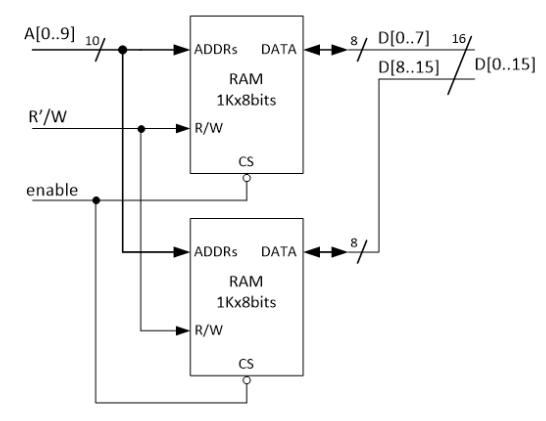
\includegraphics[scale=0.8]{img/memparalelo.png}
\end{figure}

En este ejemplo, las líneas de datos de D0 a D7 corresponden a la primera palabra de $8$ bits y las líneas de datos de D8 a D15 corresponden a la segunda palabra de $8$ bits, se juntan para formar una palabra de $16$ bits.

\subsection{Ampliación de capacidad}
Para ampliar la capacidad de una memoria, se deben agregar chips de memoria en serie y se deben conectar las líneas de dirección de manera que se seleccione el chip adecuado.

\subsubsection{Ejemplo}
En el ejemplo se debe conformar un banco de
4K direcciones, cada una de 4 bits, y para hacerlo se cuenta con chips de 1K x 4 bits. En primer lugar dividimos la capacidad total de memoria necesaria por la capacidad de cada chip, a los efectos de obtener la cantidad de chips que debemos emplear. En este caso se necesitarán 4 chips.

Se pretende aumentar la cantidad de direcciones disponibles. Cada chip posee 10 líneas de dirección, pero el banco es de 4K, o sea que necesita 12 líneas. Las líneas A0, hasta A9 (10 bits) van a todos los chips simultáneamente. Las líneas restantes (A10 y A11) entran a un decodificador cuya función es la de ir habilitando uno a uno, a los diferentes chips de memorias del banco, con el objeto de evitar un conflicto en el Bus de Datos. De este modo, sólo un chip por vez estará activo, quedando el resto, en alta impedancia, con lo que cada chip pondrá, o recibirá, datos del bus de datos en forma individual.

Lo vamos a representar con una tabla, primero tendremos el chip, cada chip tiene las direcciones que tomará, y luego las líneas de dirección que se le asignan. Podemos notar que como se busca tener 4K direcciones, se necesitan 12 líneas de dirección.

\begin{figure}[h]
    \centering
    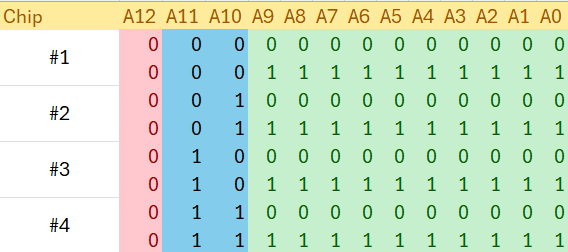
\includegraphics[scale=0.8]{img/tabla.png}
\end{figure}
Se puede observar que el banco funcionará siempre que A12 sea 0, ya que en caso contrario se generarían espejos. Luego la parte verde son las líneas de dirección que comparten todos los chips, y la parte azul son las líneas de dirección que se le asignan a cada chip. Es decir las que usaremos para seleccionar el chip que queremos leer o escribir. Para ello podemos notar que usar un decodificador de 2x4 nos permitirá seleccionar el chip que queremos leer o escribir.

\begin{figure}[h]
    \centering
    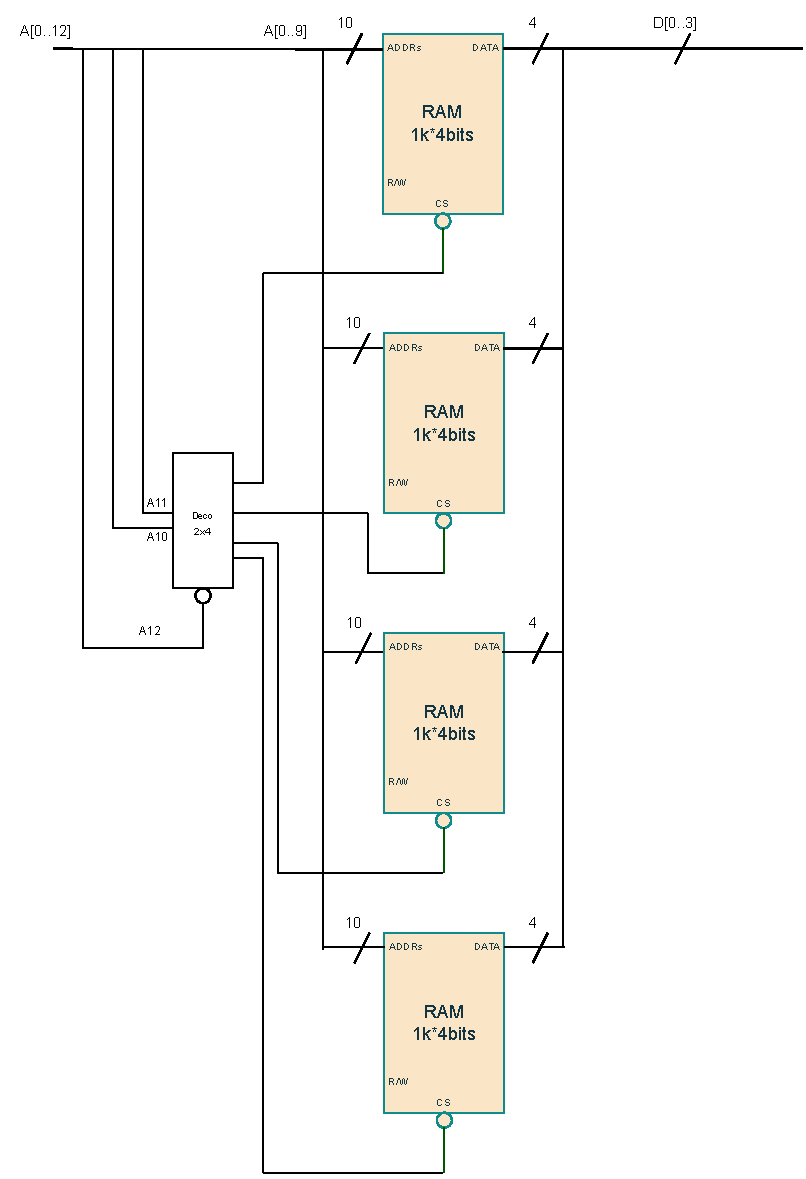
\includegraphics[scale=0.8]{img/ejmemorias.pdf}
\end{figure}
%-------------------------------------------------%


\newpage
%-- Direccionamiento y lógica de Decodificación de Memorias --%
\section{Direccionamiento y Lógica de Decodificación de Memorias}\label{sec:mem}

Una unidad de memoria es un conjunto de celdas de almacenamiento junto con los circuitos asociados que se requieren para transferir información al y del dispositivo. El tiempo que toma transferir información a o de cualquier posición al azar deseada siempre es el mismo, de ahí el nombre memoria de acceso aleatorio o RAM

Una unidad de memoria almacena información binaria en grupos de bits llamados \textbf{palabras}. Una palabra de memoria es una \textit{entidad de bits que siempre se guardan o sacan juntos}, como una unidad. Una palabra de memoria es un \textit{grupo de unos y ceros y podría representar un número, una instrucción, uno o más caracteres alfanuméricos o cualquier otra información codificada en binario}. Un grupo de ocho bits es un byte. Casi todas las memorias de computadora manejan palabras \textbf{cuya longitud es un múltiplo de ocho bits}. Así, una palabra de 16 bits contiene dos bytes, y una de 32 bits consta de cuatro bytes. La capacidad de una unidad de memoria por lo regular se da como el número total de bytes que es capaz de guardar.

\subsection{Comunicación con la Memoria}
La comunicación entre la memoria y su entorno se efectúa a través de líneas de entrada y salida de datos, líneas de selección de direcciones y líneas de control que especifican la dirección de la transferencia.

Las $n$ líneas de entrada de datos alimentan la información que se guardará en la memoria, y las $n$ líneas de salida de datos proporcionan la información que viene de la memoria. Las $k$ líneas de dirección especifican la palabra específica escogida, de entre muchas disponibles. Las dos entradas de control especifican la dirección de la transferencia deseada: la entrada de escritura hace que se transfieran datos binarios a la memoria; la de lectura hace que se saquen datos binarios de la memoria.

\begin{figure}[h]
\centering
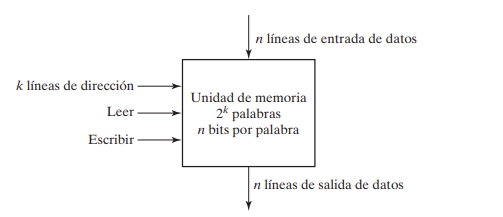
\includegraphics[scale=0.95]{img/mem.png}
\caption{Diagrama de bloques - Unidad de Memoria}
\end{figure}

La unidad de memoria se especifica con el número de palabras que contiene y el número de bits que hay en cada palabra. Las líneas de dirección seleccionan una palabra específica. A cada palabra de la memoria se asigna un número de identificación, llamado dirección, entre $0$ y $2^k -1$, donde $k$ es el número de líneas de dirección. La selección de una palabra específica de la memoria se efectúa aplicando los $k$ bits de dirección a las líneas de dirección. Un decodificador acepta esta dirección y abre las trayectorias necesarias para seleccionar la palabra especificada.

Para nombrar a las memorias, se suele decir que es de una capacidad y de tantos bits. La capacidad de palabras (o bytes) de la memoria se da con letras tales como: $K$ (kilo), $M$ (mega), $G$ (giga), $T$ (tera). $K$ es igual a $2^{10}$, $M$ es igual a $2^{20}$, $G$ es igual a $2^{30}$ y $T$ es igual a $2^{40}$.

\begin{mdframed}[backgroundcolor=gray!10,linewidth=0]
    Por ejemplo, la unidad de memoria con capacidad de 1K palabras de 16 bits cada una. Puesto que 1K=1024=210 y 16 bits constituyen dos bytes, se afirma que la memoria puede dar cabida a 2048=2K bytes.
\end{mdframed}

\newpage
El diagrama correspondiente a una memoria de $1K$ palabras de $16$ bits cada una se muestra en la figura \ref{fig:memfoto}.
\begin{figure}[h]
\centering
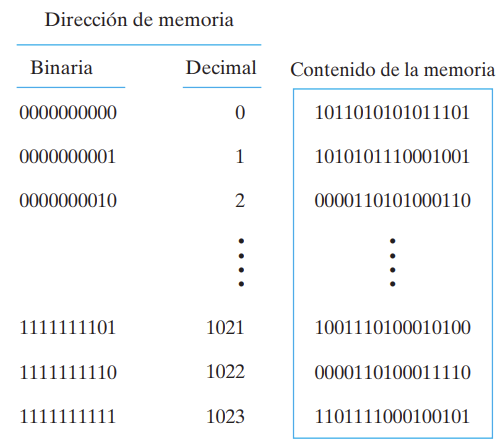
\includegraphics[scale=0.7]{img/ejem.png}
\caption{Contenido de una memoria de 1024 x 16}
\label{fig:memfoto}
\end{figure}

Cada palabra contiene 16 bits que se
dividen en dos bytes. Las palabras se reconocen por su dirección decimal, de 0 a 1023. La dirección binaria equivalente consta de 10 bits. La primera dirección se especifica con 10 ceros, y la última, con 10 unos. Ello se debe a que 1023 en binario es 1111111111. Seleccionamos una palabra de memoria por su dirección binaria. Cuando se lee o escribe una palabra, la memoria opera sobre los 16 bits como una sola unidad.

\begin{mdframed}[backgroundcolor=gray!10,linewidth=0]
    La memoria de $1K \times 16$ de la figura \ref{fig:memfoto} tiene $10$ bits en la dirección y $16$ bits en cada palabra.
\end{mdframed}

\subsection{Mapas de Karnaugh}
\begin{mdframed}[backgroundcolor=gray!10,linewidth=0]
    Los mapas de Karnaugh son una herramienta útil que nos permite aplicar un método de simplificación de funciones lógicas.
\end{mdframed}

El Mapa de Karnaugh tiene la característica de que puede ser visto como una representación bidimensional de una tabla de verdad. En la tabla de verdad, se colocan las variables por columnas y las combinaciones de tales variables determinan un valor de salida, 0 o 1, sin embargo, en el mapa las variables se colocan como si de un plano cartesiano se tratara, respetando cada una de las combinaciones que de ellas se generan, y colocando en la intersección de las combinaciones de las variables, el valor de salida.


\newpage
\begin{figure}[h]
    \centering
    \begin{karnaugh-map}[4][4][1][$w$][$z$][$y$][$x$]
        \minterms{0,1,2,3,4,8,9,11,12}
        \autoterms[0]
        \implicant{0}{8}{red}
        \implicant{0}{2}{blue}
        \implicant{0}{1}{green}
    \end{karnaugh-map}
    \caption{Ejemplo de un mapa de Karnaugh}
\end{figure}

Los mapas muestran la relación que existe entre  las entradas y las salidas de un circuito lógico, si se aplica adecuadamente el resultado será el más simplificado posible. Pueden ser utilizados para cualquier número de variables de entrada sin embargo se recomienda un máximo de seis variables.

\subsubsection{Representación de tabla de verdad en un mapa de Karnaugh}

Las tablas de la verdad se pueden representar en un mapa de Karnaugh, para ello se deben seguir los siguientes pasos:
\begin{enumerate}
    \item Se deben identificar los términos de la tabla de verdad que son 1.
    \item Se deben identificar los términos de la tabla de verdad que son 0.
    \item Se deben identificar los términos de la tabla de verdad que son 1 y que se pueden agrupar.
    \item Se deben identificar los términos de la tabla de verdad que son 0 y que se pueden agrupar.
\end{enumerate}

\begin{mdframed}[backgroundcolor=gray!10,linewidth=0]
    Observaciones:
    \begin{itemize}
        \item Los términos de la tabla de verdad que son 1 se representan en el mapa de Karnaugh con un $1$, y sirven para expresar a la función como una suma de productos.
        \item Los términos de la tabla de verdad que son 0 se representan en el mapa de Karnaugh con un $0$ y sirven para expresar a la función como un producto de sumas.
    \end{itemize}
\end{mdframed}

\newpage
\subsubsection{Ejemplo de representación de tabla de verdad en un mapa de Karnaugh}

Supongamos que se tiene la siguiente tabla de la verdad:

\begin{table}[h]
    \centering
    \begin{tabular}{ccccc}
        \toprule
        \textbf{x} & \textbf{y} & \textbf{z} & \textbf{w} & \textbf{S}\\
        \midrule
        0 & 0 & 0 & 0 & 0\\
        0 & 0 & 0 & 1 & 1\\
        0 & 0 & 1 & 0 & 1\\
        0 & 0 & 1 & 1 & 0\\
        0 & 1 & 0 & 0 & 1\\
        0 & 1 & 0 & 1 & 0\\
        0 & 1 & 1 & 0 & 0\\
        0 & 1 & 1 & 1 & 1\\
        1 & 0 & 0 & 0 & 1\\
        1 & 0 & 0 & 1 & 0\\
        1 & 0 & 1 & 0 & 0\\
        1 & 0 & 1 & 1 & 1\\
        1 & 1 & 0 & 0 & 0\\
        1 & 1 & 0 & 1 & 1\\
        1 & 1 & 1 & 0 & 1\\
        1 & 1 & 1 & 1 & 0\\
        \bottomrule
    \end{tabular}
\end{table}
Para hacer un mapa de Karnaugh, primero se separan las variabes $xy$ y $zw$ y se colocan en el mapa de la siguiente forma:

\begin{figure}[h]
    \centering
    \begin{karnaugh-map}[4][4][1][$w$][$z$][$y$][$x$]
        %\minterms{3,4,5,6,7,9,12,13,14}
        \autoterms[-]
    \end{karnaugh-map}
    \caption{Mapa de Karnaugh para las variables $xy$}
\end{figure}

\newpage
Luego identificamos los términos de la tabla de verdad que son 1 y los colocamos en el mapa de Karnaugh.
\newline Por ejemplo esta linea de la tabla
\begin{table}[h]
    \centering
    \begin{tabular}{ccccc}
        \toprule
        \textbf{x} & \textbf{y} & \textbf{z} & \textbf{w} & \textbf{S}\\
        \midrule
        0 & 0 & 0 & 1 & 1\\
        \bottomrule
    \end{tabular}
\end{table}

Se coloca en el mapa de Karnaugh en la posición donde $xy$ toma $00$ y $zw$ toma $01$.

\begin{figure}[h]
    \centering
    \begin{karnaugh-map}[4][4][1][$w$][$z$][$y$][$x$]
        \minterms{1}
        \autoterms[0]
        \implicant{1}{1}{red}
    \end{karnaugh-map}
    \caption{Ejemplo de representación}
\end{figure}

Pasar por cada linea de la tabla de verdad y colocar los términos en el mapa de Karnaugh. Los términos que no son $1$ se colocan como $0$ en el mapa de Karnaugh.

\begin{figure}[h]
    \centering
    \begin{karnaugh-map}[4][4][1][$x$][$y$][$z$][$w$]
        \minterms{1,2,4,7,8,11,13,14}
        \autoterms[0]
    \end{karnaugh-map}
    \caption{Mapa de Karnaugh completo del ejemplo.}
\end{figure}

\subsubsection{Agrupación de términos}

Para simplificar la función lógica, se deben agrupar los términos que son 1 en el mapa de Karnaugh. Los términos se pueden agrupar siguiendo las siguientes reglas:

\begin{enumerate}
    \item Los grupos deben contener una cantidad de elementos igual a potencias de 2. Es decir, los grupos solo podrán realizarse con cantidades de celdas iguales a: 1, 2, 4, 8, 16, 32, etc.
    \item Se deben generar grupos con combinaciones de variables adyacentes, es decir, sólo debe de haber un cambio entre cada una de las combinaciones, por ejemplo la combinación $ABC'$ es adyacente con $AB'C'$ , ya que sólo cambia la variable $B$.
    \item Grupos en las posiciones en los extremos y esquinas del mapa. Las posiciones de los extremos y las esquinas son adyacentes, por lo que se pueden agrupar. Esta adyacencia se debe a que el mapa de Karnaught puede ser visto como un toroide.
    \item Grupos de unos darán lugar a una suma de productos o mini términos.
    \item Grupos de ceros darán lugar a un producto de sumas o maxi términos.
    \item Los grupos deben ser lo más grande posible. Se buscará realizar grupos con la mayor cantidad de elementos posibles, entre más grande el grupo, se obtiene una función más simplificada. 
    \item No se pueden generar grupos en diagonal. Solo se permitirán grupos en vertical y horizontal dentro del mapa.
    \item Puede existir solapamiento de grupos, siempre y cuando exista al menos un elemento que no haya sido agrupado anteriormente.
    \item No deben existir grupos redundantes, es decir, no se puede realizar un grupo dentro de otro grupo, y no se puede realizar un grupo con elementos que ya hayan sido completamente agrupados en otros conjuntos.
\end{enumerate}

Por ejemplo, si se tiene este mapa de Karnaugh:

\begin{figure}[h]
    \centering
    \begin{karnaugh-map}[4][4][1][$x$][$y$][$z$][$w$]
        \minterms{4,12,6,14,0,2}
        \autoterms[0]
    \end{karnaugh-map}
    \caption{Mapa de Karnaugh para agrupar.}
\end{figure}

Se debería agrupar de la siguiente forma:

\begin{figure}[h]
    \centering
    \begin{karnaugh-map}[4][4][1][$w$][$z$][$y$][$x$]
        \minterms{4,12,6,14,0,2}
        \autoterms[0]
        \implicantedge{0}{4}{2}{6}{green}
        \implicantedge{4}{12}{6}{14}{red}
    \end{karnaugh-map}
    \caption{Mapa de Karnaugh agrupado.}
    \label{fig:karnaugh_agrupado}
\end{figure}

\newpage
\subsubsection{Simplificación de la función lógica}
Para la simplificación de la función lógica, se usan los grupos que se han formado en el mapa de Karnaugh. Cada grupo se convierte en un término de la función lógica, y se deben sumar los términos que se obtienen de los grupos, teniendo en cuenta lo siguiente:

\begin{enumerate}
    \item Si un grupo es de una sola celda, se incluye igualmente en la función lógica.
    \item En el grupo, las variables que cambian de valor "se me van" del término, y las que no cambian su valor permanecen.
    \item Si un grupo se solapa con otro, no cambia la forma de trabajarlos, cada grupo es un término distinto.
\end{enumerate}

Por ejemplo, tomando el mapa de Karnaugh anterior, se obtiene la siguiente función lógica:
\begin{equation*}
    F = x'w' + yw'
\end{equation*}


\subsection{PLA (Programmable Logic Array)}
Programmable Logic Array (PLA) es un dispositivo lógico de arquitectura fija con puertas AND programables seguidas de puertas OR programables. PLA es básicamente un tipo de dispositivo lógico programable que se utiliza para construir un circuito digital reconfigurable. La estructura de un PLA es la siguiente:

\begin{figure}[h]
    \centering
    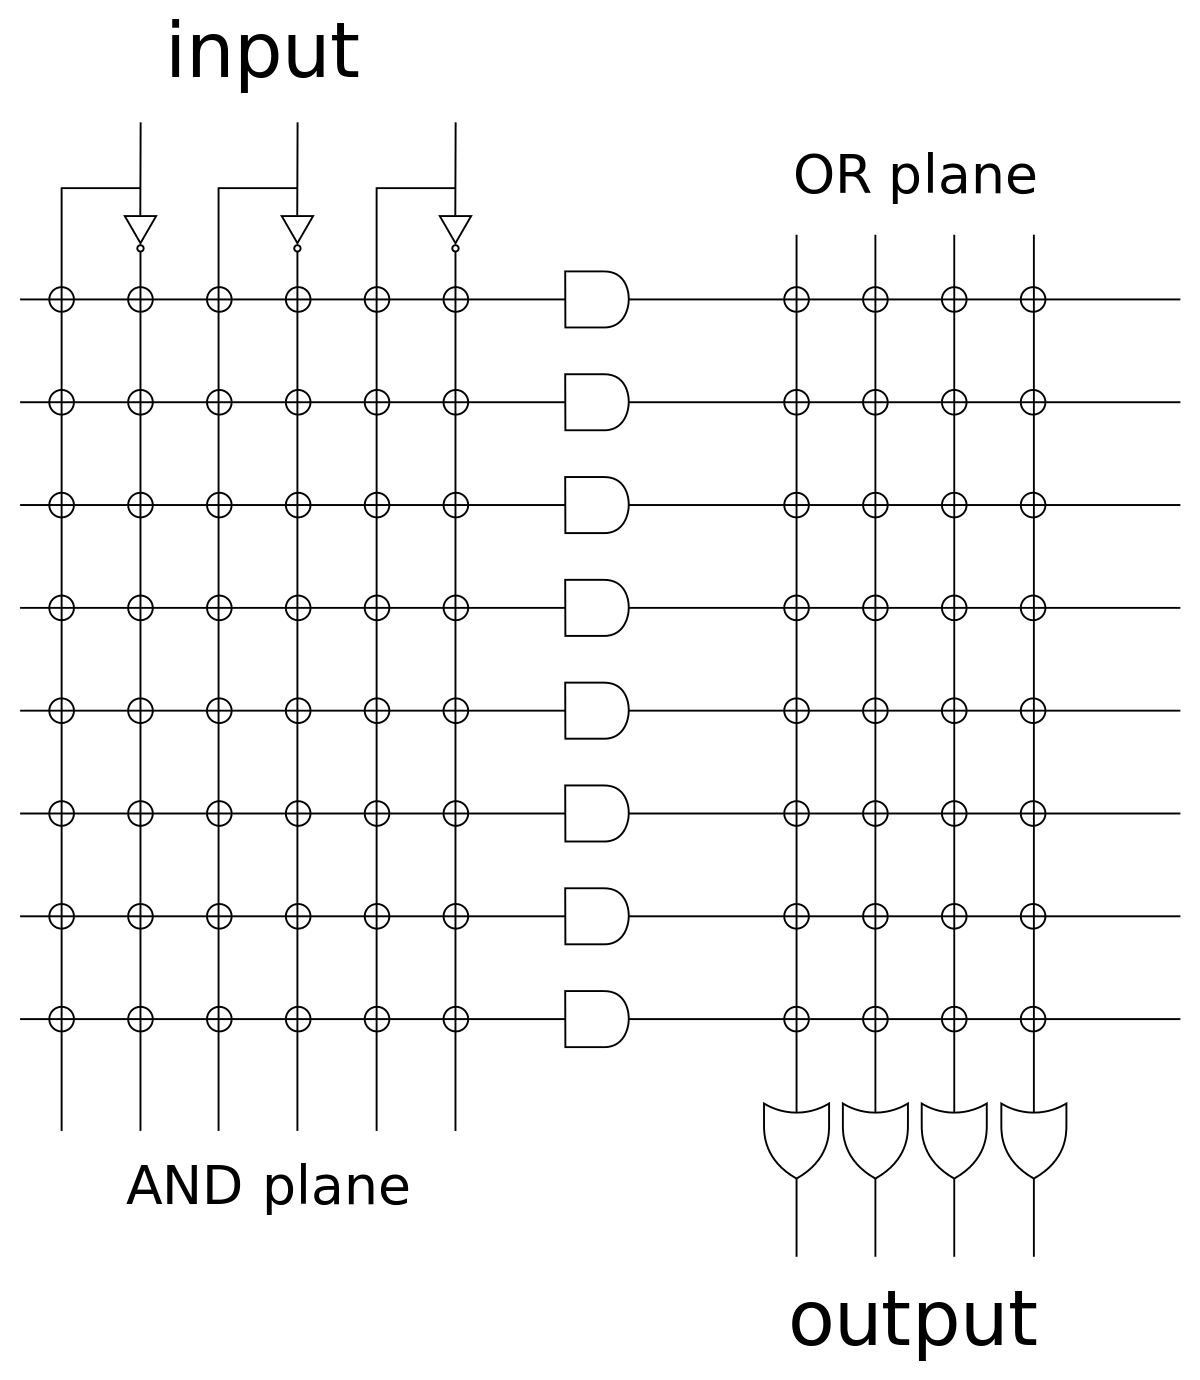
\includegraphics[scale=0.2]{img/pla.png}
    \caption{Estructura de un PLA}
\end{figure}

El funcionamiento se podria resumir en tres pasos:

\begin{enumerate}
    \item \textbf{Programación:} el usuario define la función lógica que se desea implementar.
    \item \textbf{Generación de términos del producto:} las entradas se aplican a la matriz de puertas AND para producir un conjunto de términos de producto.
    \item \textbf{Generación de suma de términos:} los términos de producto se aplican a la matriz de puertas OR para producir la salida.
\end{enumerate}

\newpage
\subsubsection{Método para implementar una función lógica en un PLA}
\begin{mdframed}[backgroundcolor=gray!10,linewidth=0]
    \begin{enumerate}
        \item Una vez se tenga la función lógica simplificada, se deben identificar los términos de la función.
        \item Cada término de la función se convierte en una fila de la matriz de puertas AND.
        \item Luego se suman los términos de la función y se convierten en una fila de la matriz de puertas OR.
        \item La salida de la matriz de puertas OR es la función lógica implementada en el PLA.
    \end{enumerate}
\end{mdframed}


\subsection{Construcción de memorias}
Cuando surge la pregunta: ¿Cuantos chips de memoria se necesitan para almacenar $1K$ palabras de $16$ bits cada una? La respuesta es: $1K \times 16 = 16K$ bits. Si cada chip de memoria tiene $1K$ bits, entonces se necesitan $16$ chips.

\begin{mdframed}[backgroundcolor=gray!10,linewidth=0]
    Para generalizar, si se tienen $m$ palabras de $n$ bits cada una, se necesitan $m \times n$ bits. Si cada chip de memoria tiene $k$ bits, entonces se necesitan $\frac{m \times n}{k}$ chips.
\end{mdframed}

\newpage
\subsubsection{Tamaño de la memoria y dirección}
La cantidad de bits de una memoria se calcula como $2^{\text{dirección}} \times \text{tamaño de palabra}$. Por ejemplo, si se tiene una memoria de $16$ palabras de $8$ bits cada una, la cantidad de bits de la memoria es $2^4 \times 8 = 128$ bits. 

Generalmente el gráfico de una memoria se representa de la siguiente manera:

\begin{figure}[h]
    \centering
    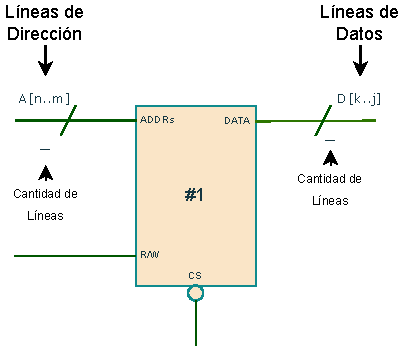
\includegraphics[scale=1]{img/diagramamem.pdf}
    \caption{Diagrama de una memoria}
\end{figure}
Donde de la cantidad de líneas de dirección se obtiene la cantidad de palabras y de la cantidad de líneas de datos se obtiene el tamaño de la palabra.


\subsection{Ampliación de palabra}
Para ampliar la palabra de una memoria, se debe agregar un chip de memoria adicional. Por ejemplo, si se tiene una memoria de $1k$ palabras de $8$ bits cada una y se desea ampliar la palabra a $16$ bits, se debe agregar un chip de memoria adicional.

\begin{figure}[h]
    \centering
    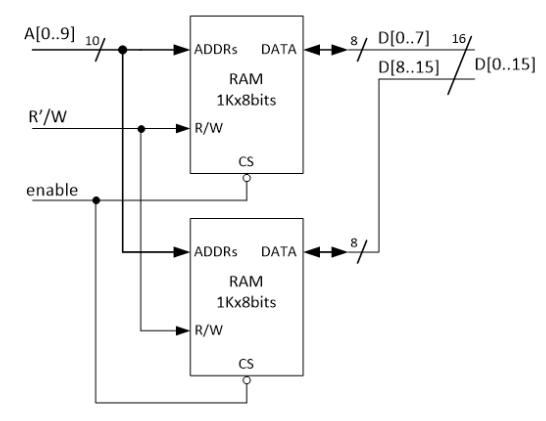
\includegraphics[scale=0.8]{img/memparalelo.png}
\end{figure}

En este ejemplo, las líneas de datos de D0 a D7 corresponden a la primera palabra de $8$ bits y las líneas de datos de D8 a D15 corresponden a la segunda palabra de $8$ bits, se juntan para formar una palabra de $16$ bits.

\subsection{Ampliación de capacidad}
Para ampliar la capacidad de una memoria, se deben agregar chips de memoria en serie y se deben conectar las líneas de dirección de manera que se seleccione el chip adecuado.

\subsubsection{Ejemplo}
En el ejemplo se debe conformar un banco de
4K direcciones, cada una de 4 bits, y para hacerlo se cuenta con chips de 1K x 4 bits. En primer lugar dividimos la capacidad total de memoria necesaria por la capacidad de cada chip, a los efectos de obtener la cantidad de chips que debemos emplear. En este caso se necesitarán 4 chips.

Se pretende aumentar la cantidad de direcciones disponibles. Cada chip posee 10 líneas de dirección, pero el banco es de 4K, o sea que necesita 12 líneas. Las líneas A0, hasta A9 (10 bits) van a todos los chips simultáneamente. Las líneas restantes (A10 y A11) entran a un decodificador cuya función es la de ir habilitando uno a uno, a los diferentes chips de memorias del banco, con el objeto de evitar un conflicto en el Bus de Datos. De este modo, sólo un chip por vez estará activo, quedando el resto, en alta impedancia, con lo que cada chip pondrá, o recibirá, datos del bus de datos en forma individual.

Lo vamos a representar con una tabla, primero tendremos el chip, cada chip tiene las direcciones que tomará, y luego las líneas de dirección que se le asignan. Podemos notar que como se busca tener 4K direcciones, se necesitan 12 líneas de dirección.

\begin{figure}[h]
    \centering
    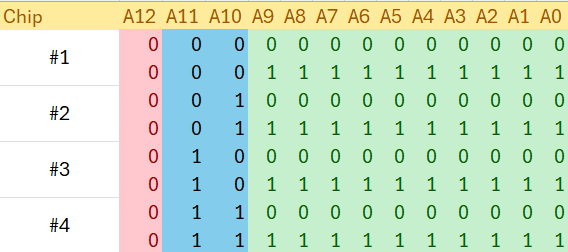
\includegraphics[scale=0.8]{img/tabla.png}
\end{figure}
Se puede observar que el banco funcionará siempre que A12 sea 0, ya que en caso contrario se generarían espejos. Luego la parte verde son las líneas de dirección que comparten todos los chips, y la parte azul son las líneas de dirección que se le asignan a cada chip. Es decir las que usaremos para seleccionar el chip que queremos leer o escribir. Para ello podemos notar que usar un decodificador de 2x4 nos permitirá seleccionar el chip que queremos leer o escribir.

\begin{figure}[h]
    \centering
    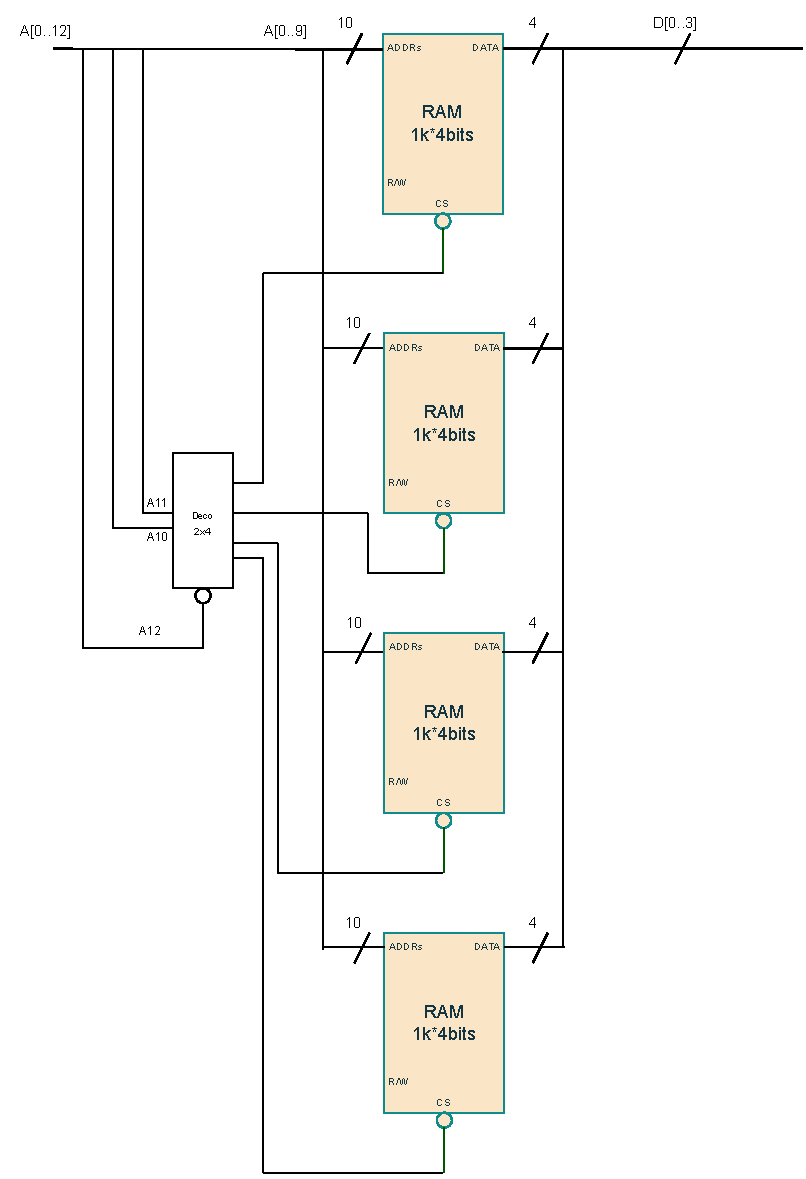
\includegraphics[scale=0.8]{img/ejmemorias.pdf}
\end{figure}
%-------------------------------------------------%

\newpage
%-------------- Circuitos Secuenciales --------------%
\section{Circuitos Secuenciales}\label{sec:sec}

\documentclass[20pt,margin=1in,innermargin=-4.5in,blockverticalspace=-0.25in]{tikzposter}
\geometry{paperwidth=42in,paperheight=30in}
\usepackage[utf8]{inputenc}
\usepackage{amsmath}
\usepackage{amsfonts}
\usepackage{amsthm}
\usepackage{amssymb}
\usepackage{mathrsfs}
\usepackage{graphicx}
\usepackage{adjustbox}
\usepackage{enumitem}
\usepackage[backend=biber,style=numeric]{biblatex}
\usepackage{emory-theme}
\usepackage{emory-theme}
\usepackage{mwe} % for placeholder images
\usepackage{booktabs}
% set theme parameters
\tikzposterlatexaffectionproofoff
\usetheme{EmoryTheme}
\usecolorstyle{EmoryStyle}

\title{Sistema IEEE 754 - Precisión Simple}
\author{Pedro Villar}
\institute{Organización del Computador - Primer Cuatrimestre 2024}	
\titlegraphic{\adjustbox{left=0.35\textwidth}{
\includegraphics[width=0.3\textwidth]{famaf-logo.jpg}}}

% begin document
\begin{document}
\maketitle
\centering
\block{¿Qué es el sistema IEEE 754?}{
        El sistema IEEE 754 es un estándar para la representación de números en punto flotante. Este sistema establece las caracteristicas de las tres partes de un número en punto flotante: el \textbf{signo}, \textbf{exponente} y \textbf{fracción (mantisa)}. Se enfoca en el método de precisión simple que utiliza 32 bits.
    }
\begin{columns}
    \column{0.5}
    \block{Características}{
        \begin{center} \textbf{Bit de signo:} \end{center}
        El bit de signo es el primer bit del número en punto flotante. \textbf{Si el bit de signo es 0}, el número es \textbf{positivo}, \textbf{si es 1}, el número es \textbf{negativo}.    
        \begin{center} \textbf{Exponente:} \end{center}
        Indica cuántos “lugares” se debe desplazar hacia la derecha o hacia la izquierda la coma binaria de la parte significativa. El exponente de un número puede ser tanto positivo como negativo. En el caso de la precisión simple, el exponente se representa con 8 bits y se suma 127 al valor del exponente para obtener el valor.
        \begin{center} \textbf{Mantisa o parte fraccionaria:} \end{center}
        La mantisa es la parte fraccionaria del número en punto flotante. En el caso de la precisión simple, la mantisa se representa con 23 bits. Debe ser normalizada, eso se logra moviendo la coma binaria a la izquierda hasta que el primer bit sea 1.
        \begin{equation*}
            1,xxxxx \times 2^{yyyy}
        \end{equation*}
        Al hacer esto, se debe adaptar el exponente para que el valor no se modifique, es decir, el exponente será ahora \textbf{la cantidad de veces que se movió la coma binaria a la izquierda}.
    }

    \block{Convertir de decimal a IEEE 754}{
        \begin{enumerate}
            \item Determinar el bit de signo.
            \item Convertir la parte entera y la parte fraccionaria a binario.
            \item Normalizar.
            \item Encontrar el exponente moviendo la coma y sumando 127, expresado en binario.
            \item Encontrar la parte fraccionaria.
            \item Conformar el número en punto flotante.
        \end{enumerate}
    }
    \block{Convertir de IEEE 754 a decimal}{
        \begin{enumerate}
            \item Dividir el número en punto flotante en sus tres partes.
            \item Encontrar el bit de signo.
            \item Encontrar el exponente y restarle 127.
            \item Desnormalizar el número y pasarlo a decimal.
        \end{enumerate}
    }
    
    \column{0.5}
    \block{Ejemplo de conversión de decimal a IEEE 754}{
        Se busca convertir el número $723.125_{10}$ a IEEE 754.
        \begin{enumerate}
            \item El bit de signo es 0, ya que el número es positivo.
            \item Se convierte la parte entera y la parte fraccionaria a binario.
            \begin{itemize}
                \item Parte entera:
                \begin{align*}
                    723 \div 2 &= 361 \text{ residuo } 1 \\
                    361 \div 2 &= 180 \text{ residuo } 1 \\
                    180 \div 2 &= 90 \text{ residuo } 0 \\
                    90 \div 2 &= 45 \text{ residuo } 0 \\
                    45 \div 2 &= 22 \text{ residuo } 1 \\
                    22 \div 2 &= 11 \text{ residuo } 0 \\
                    11 \div 2 &= 5 \text{ residuo } 1 \\
                    5 \div 2 &= 2 \text{ residuo } 1 \\
                    2 \div 2 &= 1 \text{ residuo } 0 \\
                    1 \div 2 &= 0 \text{ residuo } 1 \\
                \end{align*}
                Por lo que la parte entera en binario es $1011010011$.
                \item Parte fraccionaria:
                \begin{align*}
                    0.125 \times 2 &= 0.25 \\
                    0.25 \times 2 &= 0.5 \\
                    0.5 \times 2 &= 1
                \end{align*}
                Por lo que la parte fraccionaria en binario es $001$.
            \end{itemize}
            El número en binario es $1011010011.001$.
            \item Para normalizar movemos la coma tantos lugares como sea necesario para que quede un uno seguido por una parte fraccionaria.
            \begin{itemize}
                \item \textbf{Sin normalizar:} $1011010011.001 \times 2^0$
                \item \textbf{Normalizado:} $1.011010011001 \times 2^{10}$
            \end{itemize}
            \item El exponente es la cantidad de veces que se movió la coma binaria a la izquierda, en este caso, 10 veces. Por lo que el exponente es $127 + 10 = 137_{10} = 10001001_2$.
            \item La parte fraccionaria se compone por los 23 bits que siguen a la coma decimal del número normalizado.
            \begin{equation*}
                01101001100100000000000
            \end{equation*}
            \item Para conformar el número en punto flotante, se coloca el bit de signo, el exponente y la parte fraccionaria.
            \begin{equation*}
                0 \ 10001001 \ 01101001100100000000000
            \end{equation*}
        \end{enumerate}   
    }
\end{columns}

\end{document}
%-------------------------------------------------%

\end{document}